\documentclass[12pt, letterpaper]{article}
\usepackage[utf8]{inputenc}
\usepackage{hyperref}
\usepackage{enumerate}
\usepackage{listings}
\usepackage{fancyvrb}

\usepackage{tikz}
\usepackage{graphicx}
\usetikzlibrary{positioning}

\usepackage[document]{ragged2e} % keep all left
\usepackage{minted} % yaml syntax highlighting

\newenvironment{markdown}%
    {\VerbatimEnvironment\begin{VerbatimOut}{tmp.markdown}}%
    {\end{VerbatimOut}%
        \immediate\write18{pandoc tmp.markdown -t latex -o tmp.tex}%
        \input{tmp.tex}}

\providecommand{\tightlist}{%
  \setlength{\itemsep}{0pt}\setlength{\parskip}{0pt}}

\newcommand*{\email}[1]{\href{mailto:#1}{\nolinkurl{#1}} } 

\title{Kubernetes Workshop \\{\small \href{https://creativecommons.org/licenses/by/4.0/}{CC BY 4.0} }  }
\author{Wojciech Barczynski (wbarczynski.pro@gmail.com)}
\date{}

\usepackage{pmboxdraw} % verbatim and unicode https://tex.stackexchange.com/questions/245777/latex-and-unicode-within-verbatim-environment

\begin{document}

\begin{titlepage}
\maketitle
\end{titlepage}

\tableofcontents
\pagebreak
\section{Prerequiments}

You need to feel good with Command Line Interface. You should understand what Docker is.

\begin{itemize}%
\item Workstation with Linux or OSX recommended.%
\item Software \begin{itemize}%
    \item k3s
    \item Kubernetes {\small CLI}
    \item Docker
    \end{itemize}%
\item Tools \begin{itemize}%
    \item jq (\href{https://stedolan.github.io/jq/}{stedolan.github.io/jq/})%
    \end{itemize}
\item Good to have \begin{itemize}%
    \item hub.docker.com account or alternative docker repository
    \end{itemize}
\end{itemize}

\subsection{How to install}

\begin{markdown}
- K3S - [github.com/k3s-io/k3s](https://github.com/k3s-io/k3s)
- Kubernes CLI - [kubernetes.io/docs/tasks/tools/](https://kubernetes.io/docs/tasks/tools/)
\end{markdown}

\subsection{Verify the setup}

% --port "8443:8443@loadbalancer" 
% https://k3d.io/usage/guides/exposing_services/
\begin{verbatim}
$ k3d cluster create --port "8080:8080@loadbalancer" \
                     --port "8000:80@loadbalancer" \
                     'k8s-w10i-workshop'
\end{verbatim}

\begin{verbatim}
$ kubectl config use-context k3d-k8s-w10i-workshop

$ kubectl cluster-info

Kubernetes control plane is running at https://0.0.0.0:60602
CoreDNS is running at https://...
Metrics-server is running at https://...
\end{verbatim}

\subsection{Kubernetes {\small CLI} Basics}

Let's learn first some basics regarding the \textit{kubectl}:

\begin{verbatim}
kubectl get <ARTIFACT>
kubectl describe <ARTIFACT>
\end{verbatim}

From the kubect ref
\href{https://kubernetes.io/docs/reference/kubectl/overview/}{kubernetes.io/docs/reference/kubectl/overview}:

\begin{verbatim}
kubectl [command] [TYPE] [NAME] [flags]
\end{verbatim}

\bigskip
1. List the nodes (underlaying machines or virualmachines running k8s):

\begin{verbatim}
$ kubectl get nodes
\end{verbatim}

What the names of our nodes are? . . .

\bigskip
2. Let's learn more about the node:

\begin{verbatim}
# the name of the node you saw from previous
# command
$ kubectl get nodes k3d-k8s-w10i-workshop-server-0
$ kubectl get nodes k3d-k8s-w10i-workshop-server-0 -o wide

# notice:
#   most of services have shortnames:
$ kubectl get no k3d-k8s-w10i-workshop-server-0
$ kubectl get node k3d-k8s-w10i-workshop-server-0
$ kubectl get nodes k3d-k8s-w10i-workshop-server-0
\end{verbatim}

You can find the abbreviations with the command: 

\begin{verbatim}
$ kubectl api-resources
\end{verbatim}

\bigskip
3. Get more details: 

\begin{verbatim}
$ kubectl describe nodes k3d-k8s-w10i-workshop-server-0
\end{verbatim}

Note down:
\begin{itemize}
    \item Container Runtime Version: . . .
    \item  What the namespaces we have: . . .
    \item  Note down name of two pods:\begin{itemize}
        \item . . .
        \item . . .
     \end{itemize}
\end{itemize}

\bigskip
4. YAML and JSON output

\begin{verbatim}
$ kubectl get node k3d-k8s-w10i-workshop-server-0 -o yaml
$ kubectl get node k3d-k8s-w10i-workshop-server-0 -o json
\end{verbatim}

Use \textit{jq} to get the \textit{kubeletVersion}, write down below:
\\

   . . .

\bigskip
5. Notice, \verb|kubectl| provides support for jsonpath:

\begin{verbatim}
$ kubectl get node k3d-k8s-w10i-workshop-server-0 \
  -o jsonpath="{.status.daemonEndpoints.kubeletEndpoint.Port}"
\end{verbatim}

\begin{verbatim}
$ kubectl get node k3d-k8s-w10i-workshop-server-0 \
  -o jsonpath="{.metadata.labels}"
\end{verbatim}

Write down a command with jsonpath to get information on how many CPU we have allocated to our minikube:
\\

   . . .


\bigskip
6. All Kubernetes resources have labels attached:

\begin{verbatim}
# show me nodes that have the following label
$ kubectl get no  -l 'kubernetes.io/hostname'

# show me nodes running on linux
$ kubectl get no  -l 'kubernetes.io/os=linux'
\end{verbatim}

Please find another label, you could select our node and run the command.

\bigskip
7. Recommendations for your local setup:

\begin{markdown}
- ```alias k=kubectl``` or ```alias kb=kubectl``` (more ideas on [github.com/prezto-contributions/prezto-kubectl](https://github.com/prezto-contributions/prezto-kubectl))
- ```kubectx``` and ```kubens``` - [github.com/ahmetb/kubectx](https://github.com/ahmetb/kubectx)


If you do not want to install kubectx, create an alias that will let you quickly check to which of kubernetes clusters, you are "connected":

```alias kctx='kubectl config current-context'```
\end{markdown}
%
%
%
\section{Kubectl configuration file}

Your kubectl configuration is in \verb|${HOME}/.kube/config|, it contains tokens, certificates, aliases etc. You will need to edit this file very seldom.%

\bigskip
1. View \verb|${HOME}/.kube/config|.

\bigskip
2. Find \textit{certificate-authority}.

\bigskip
3. Note the main sections:%

   . . .\\
   . . .\\
   . . .\\

% clusters
% contexts
% users
\pagebreak
\section{Task at Hand}

Our goal today will be deployment of \verb|intro-app| on Kubernetes. It is a simple web service. We will start with learning about the Kubernetes deployment and service as shown on the picture.

\begin{figure}[ht]
\centering
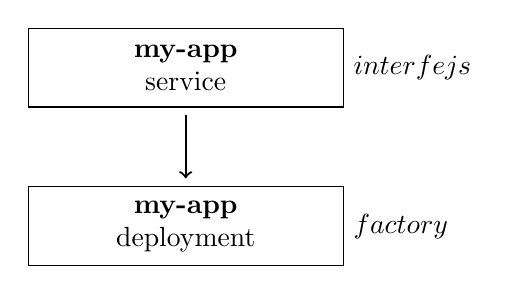
\begin{tikzpicture}
\node[draw,minimum width=4cm,minimum height=1cm, text width=2cm, align=center, label=right:$interfejs$] (S){\textbf{my-app} service};

\node[draw,minimum width=4cm,minimum height=1cm, text width=2cm, align=center, label=right:$factory$] (D) [below =of S] {\textbf{my-app} \\ deployment};

\draw [->,thick,shorten >=1mm,shorten <=1mm] (S.south) -- (D.north);

\end{tikzpicture}
\end{figure}


%We need to deploy \verb|intro-app| on kubernetes. Users will acess this application on \verb|my.app/echo|. Please help us, our next finanse round depens on it!

\section{What are the namespaces?}

\begin{verbatim}
$ kubectl get ns
$ kubectl get namespaces
\end{verbatim}

Notice:
\begin{itemize}
    \item you can create namespaces to better organize your components
    \item you might define resource restrictions per namespaces
    \item effect the name: \textit{$<$service-name$>$.$<$namespace-name$>$.svc.cluster.local}. We will talk about it later.
\end{itemize}

To change the selected namespace for our commands:

\begin{verbatim}
$ kubectl config set-context \
  $(kubectl config current-context) \
  --namespace <namespace-name>
\end{verbatim}

You can specify namespace explicitly with the kubectl {\small CLI}:

\begin{verbatim}
$ kubectl get pods --namespace=kube-system
$ kubectl get pods -n kube-system
$ kubectl get po -n default
\end{verbatim}

Notice: you can check \verb|kubectl api-resources| to see which resources are namespaced and which not.

%
%
\pagebreak
\section{Kubernetes deployments.yaml}

Let's get instances of our application running. We use an application docker image built on the top of official nginx (\href{https://hub.docker.com/\_/nginx}{hub.docker.com/\_/nginx}), you will find Dockerfiles in \texttt{manifests/dockers}.

\bigskip
0. The Kubernetes deployment resource as a factory that creates pods based on a template definition. The deployment uses labels to "find" its pods. If any pod is missing, Kubernetes will schedule missing number of pods.

\begin{figure}[ht]
\centering
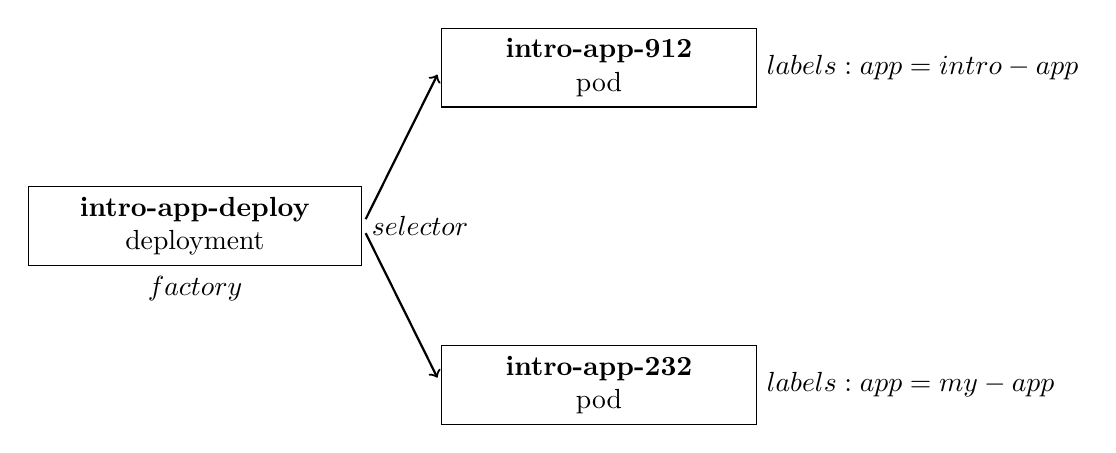
\begin{tikzpicture}
\node[draw,minimum width=4cm,minimum height=1cm, text width=4cm, align=center, label=below:$factory$, label=right:$selector$] (D){\textbf{intro-app-deploy} \\ deployment};

\node[draw,minimum width=4cm,minimum height=1cm, text width=3cm, align=center, label=right:{$labels: app=intro-app$}] (P1) [above right=of D] {\textbf{intro-app-912} \\ pod};

\node[draw,minimum width=4cm,minimum height=1cm, text width=3cm, align=center, label=right:{$labels: app=my-app$}] (P2) [below right=of D] {\textbf{intro-app-232} \\ pod};

\draw [->,thick,shorten >=1mm,shorten <=1mm] (D.east) -- (P1.west);
\draw [->,thick,shorten >=1mm,shorten <=1mm] (D.east) -- (P2.west);

\end{tikzpicture}
\end{figure}

Notice: \verb|deployment| (apps/v1) uses \verb|replicasets| (\verb|k get rs|) under the hood.

\bigskip
1. Let's understand the deployment manifest \texttt{manifests/kube-deployment.yaml}(showing a minimal manifest):

\inputminted{yaml}{manifests/kube-deployment.yaml}

\smallskip
Notice: the postfix \verb|-deploy| is not the best practise, just to make it more explicit what-is-what during the training.

\smallskip
Hints:
\begin{itemize}
\item if your repo is private, you need to define \verb|imagePullSecrets| (check official docs\footnote{\href{https://kubernetes.io/docs/tasks/configure-pod-container/pull-image-private-registry/}{kubernetes.io/docs/tasks/configure-pod-container/pull-image-private-registry/}}).
\item You can forge Kubernetes to pull Docker image every time with\\ \verb|imagePullPolicy: Always|, not recommended but might be helpful during the development. You MUST NOT use this setting in \textbf{production}.
\end{itemize}

\bigskip
2. Let's get our application running by creating the Kubernetes deployment that will start the app for us:

\begin{verbatim}
# declarative
$ kubectl apply -f manifests/kube-deployment.yaml
deployment.apps/intro-app-deploy created

# imperative way (alternative to the previous command):
$ kubectl create -f manifests/kube-deployment.yaml
deployment.apps/intro-app-deploy created
\end{verbatim}

If you want to know more about the difference, checks docs:\begin{itemize}
\item Imperative config - \href{https://kubernetes.io/docs/concepts/overview/object-management-kubectl/imperative-config/}{kubernetes.io/docs/concepts/overview/object-management-kubectl/imperative-config},
\item Declarative config - \href{https://kubernetes.io/docs/concepts/overview/object-management-kubectl/declarative-config/}{kubernetes.io/docs/concepts/overview/object-management-kubectl/declarative-config/}.
\end{itemize}

\bigskip
3. List deployments to see whether there is your deployment resource:

\begin{verbatim}
# deploy, deployment, deployments
$ kubectl get deploy

NAME               READY   UP-TO-DATE   AVAILABLE   AGE
intro-app-deploy   1/1     1            1           19s

$ kubectl get deploy -o wide
# notice the selector

\end{verbatim}

\bigskip
4. Check the details about the Kubernetes deployment:

\begin{verbatim}
$ kubectl describe deploy <DEPLOYMENT_NAME>
\end{verbatim}

Notice fields for update strategy (more about it later) and replicas.

\bigskip
5. Where is our app? The pods:

\begin{verbatim}
# "po" = "pod" or "pods"
$ kubectl get po
$ kubectl get po -n default
\end{verbatim}

\begin{verbatim}
$ kubectl describe po <POD_NAME>
\end{verbatim}

\bigskip
6. Find the following information:
\begin{itemize}
    \item How many containers are in the pod? . . .
    \item What is the IP of your app pod? . . .
    \item What is ReplicatSet? . . .
    \item Ready? . . .
    \item Restart Count? . . .
    \item Events? . . .
\end{itemize}

Notice: we will discus other fields -- QoS, Conditions (Ready), Node-Selector, and Tolerations -- later.
%
\bigskip
7. Increase the number of pods, modify the {\small YAML} manifest and apply the changes. Check wherher you see more pods \verb|kubectl get po|. If the answer is yes, please scale down your deployment to one pod instance.
%
\bigskip
8. What does it happen when you delete one of the pods? 
\begin{verbatim}
$ kubectl delete po intro-app-65db4-...
$ kubectl get po
\end{verbatim}

\section{Check whether app works with port forwarding}

We can see the app running but does it work? We did not expose our application outside the cluster, so we need another mechanism at this moment. Kubernetes provide us \verb|port-forward| to forward port from the pod to local machine port.

\bigskip
1. Find the port our application listen on\footnote{Notice: the deployment manifest does not enforce the port number the application listen on.}.

\bigskip
2. Setup the port forwarding:

\begin{verbatim}
kubectl port-forward <POD_NAME> <LOCAL_PORT_NUMBER>:<POD_PORT_NUMBER>
\end{verbatim}

\begin{verbatim}
# let's choose 8080 as the local port
$ kubectl port-forward <POD_NAME> 8080:<POD_PORT_NUMBER>

# in a separate terminal:
$ curl 127.0.0.1:8080

<html>
<h1>1.0.0</h1>
</html>

# if you prefer httpie (httpie.io)
$ http 127.0.0.1:8080
\end{verbatim}

\smallskip

You will use \verb|port-forward| very often as one of the first steps of many debugging sessions for why-client-cannot-connect-to-my-service-from-outside.

\bigskip

The \verb|port-forward| can take also as a parameter also Kubernetes service or deployment\footnote{\href{https://kubernetes.io/docs/tasks/access-application-cluster/port-forward-access-application-cluster/}{kubernetes.io/docs/tasks/access-application-cluster/port-forward-access-application-cluster}}.

\bigskip
Let's learn about services and ingresses first, later 
we see how we can modify our deployment and update the application.

\section{Get your application logs}
Let's keep the port-forwarding running and open the second terminal to examinate logs:

\begin{verbatim}
$ kubectl logs <POD NAME>

$ kubectl logs <POD NAME> -f # -f as in tail -f ;)
\end{verbatim}

Send few requests with \verb|curl| to see new entries in the logs. You will use this command a lot, so check the command help \verb|k logs --help|.

\pagebreak
\section{Opening console in your container}

Sometimes, you would like to check your appliacation from within the container. Let's see how we can achieve it with Kubernetes

\bigskip
1. Get the console:

\begin{verbatim}
# check the pod name
$ kubectl exec -it intro-app-... -- /bin/bash
\end{verbatim}

Let's print env variables:

\begin{verbatim}
$ kubectl exec -it intro-app-65d /bin/bash

root@intro#$ printenv

root@intro#$ printenv | grep DB
\end{verbatim}

\bigskip
2. Add tool for debugging - curl:

\begin{verbatim}
root@intro#$ apt-get update && apt-get install -qq curl
\end{verbatim}

\bigskip
3. Does it work?

\begin{verbatim}
# does it work?
root@intro#$ curl 127.0.0.1

# can we get outside
root@intro#$ curl -I wbarczynski.pl

# can we reach other services:
root@intro#$ telnet kube-dns.kube-system 53
\end{verbatim}

\bigskip
4. Assuming we resolve our issue, let's clean up by deleting the pod we install utilites for debugging:

\begin{verbatim}
$ kubectl delete po intro-app-65db4-...
\end{verbatim}
%
%
%
\pagebreak
\section{Kubernetes Service}

Our factory, I mean the deployment defines how we create our application instanes as pods. The service, how we expose it to be consumed. We have three types of Services: LoadBalancer, ClusterIP (the most commonly used), NodePort, and ExternalName ({\small CNAME} to an external service).

\begin{figure}[ht]
\centering
\begin{tikzpicture}
\node[draw, dashed, minimum width=4cm,minimum height=1cm, text width=4cm, align=center, label=below:$selector$, label=right:$interface$] (S){\textbf{intro-app-svc} \\ service};

\node[draw,minimum width=4cm,minimum height=1cm, text width=3cm, align=center, label=above:{$labels: app=intro-app$}] (P1) [below left=of D] {\textbf{intro-app-912} \\ pod};

\node[draw,minimum width=4cm,minimum height=1cm, text width=3cm, align=center, label=above:{$labels: app=intro-app$}] (P2) [below right=of D] {\textbf{intro-app-232} \\ pod};

\node[draw,minimum width=4cm,minimum height=1cm, text width=3cm, align=center] (C) [above=of D] {\textbf{client}};


\draw [->,thick,shorten >=1mm,shorten <=1mm] (S.south) -- (P1.north east);
\draw [->,thick,shorten >=1mm,shorten <=1mm] (S.south) -- (P2.north west);
\draw [->,thick,shorten >=1mm,shorten <=1mm] (C.south) -- (S.north);

\end{tikzpicture}
\end{figure}

\bigskip
1. Let's go through the (pretty basic) manifest \texttt{manifests/kube-service.yaml} (again the \emph{-svc} prefix for the clarity):

\inputminted{yaml}{manifests/kube-service.yaml}

\bigskip
2. Deploy:

\begin{verbatim}
$ kubectl create -f manifests/kube-service.yaml
$ kubectl apply -f manifests/kube-service.yaml
\end{verbatim}

\bigskip
3. Let's call our service through loadbalancer that we exposed on \verb|8080|:

\begin{verbatim}
# http 127.0.0.1:8080
$ curl -s -D - 127.0.0.1:8080
HTTP/1.1 200 OK
Server...

<html>
<h1>1.0.0</h1>
</html>
\end{verbatim}

Notice: on {\small AWS}, Azure, or {\small GCP}, we would get the loadbalancer created and public {\small IP} assigned. You would than use annotations to specify the loadbalancer configuration, for example:\\ \href{https://docs.aws.amazon.com/eks/latest/userguide/network-load-balancing.html}{docs.aws.amazon.com/eks/latest/userguide/network-load-balancing.html}.

\bigskip
4. Let's list the services and get more details about our newly created service:

\begin{verbatim}
$ kubectl get services
$ kubectl get svc -o wide
$ kubectl describe svc intro-app-svc
\end{verbatim}

Please note down:

\begin{markdown}
- Endpoints (where this IP comes from?) . . . 
- Selector . . .
- IP . . .
\end{markdown}

\bigskip
5. Short recap with the trainer - service types:

\begin{markdown}
- ClusterIP with and without IP (headless)
- LoadBalanced
- ExternalName
\end{markdown}

\bigskip
6. How does the service work? Let's use busybox\footnote{"The Swiss Army Knife of Embedded Linux" - \href{https://hub.docker.com/_/busybox}{\url{hub.docker.com/_/busybox}} } docker to see how we can access the service from a different app.

\begin{verbatim}
$ kubectl run busybox --image=busybox:1.28.4 --rm \
    --restart=OnFailure -ti -- /bin/nslookup intro-app-svc

$ kubectl run -i --tty busybox-wget --rm \
    --image=busybox:1.28.4 -- sh

/# wget -O- intro-app-svc
/# wget -O- intro-app-svc.default
/# wget -O- intro-app-svc.default.svc
/# wget -O- kubernetes-dashboard.kube-system
\end{verbatim}%

By the way, the service info is also injected as environment variables. I did not have so far a need to use this information:%
\begin{verbatim}
$ kubectl run busybox --image=busybox \
  --rm --restart=OnFailure -ti -- printenv | grep -i intro_app_svc
\end{verbatim}%

You could also run nslookup from within our app pods:%
\begin{verbatim}
$ kubectl exec -it intro-app-deploy-5d556d9f4b-vslp9 \
    -- /bin/bash

/# apt-get update && apt-get install dnsutils -qq
/# nslookup intro-app-svc
\end{verbatim}%

\bigskip
7. You will use ClusterIP service with Ingress controller more often than Loadbalancer service.

%
\section{Modyfing kubernetes deployment and service}

Avoid editing files on kubernetes, always modify a yaml and apply the changes.

\bigskip
1. Change the number of pods running to 2 with:

\begin{verbatim}
$ kubectl edit deploy
\end{verbatim}

\begin{verbatim}
$ kubectl get po
\end{verbatim}

\bigskip
2. Change the value of label \verb|me| to your name in the service definition.

\bigskip
3. Modify the \verb|depoyment.yml| to get 3 pods, use: \texttt{kubectl apply -f}

\bigskip
4. Add one more label to service.

\bigskip
5. What does happen if we add one more selector, apply it:

\inputminted{yaml}{manifests/exercise-broke-svc/kube-service-broke.yml}

Can we connect?

\begin{verbatim}
# again, let's connect through LB
$ curl -s -D - 127.0.0.1:8080

\end{verbatim}

What has changed?
\begin{verbatim}
$ kubectl describe svc intro-app-svc
\end{verbatim}

\bigskip
Notice: {\large very very very common issue} that selectors do not match labels.

\bigskip
6. Fix your service.

%
%
%
\section{Updating service}

Let's update our app from the version \verb|1.0.0| to \verb|2.0.0|:

\bigskip
1. Change in the deployment file and apply changes.

\bigskip
2. You can also change it with set image:

\begin{verbatim}
$ kubectl set image deployment/<DEPLOYMENT_NAME> \
  <CONTAINER_NAME>=<DOCKER_IMAGE_NAME>:<VERSION>
\end{verbatim}

\bigskip
3. Change two times from \verb|1.0.0| to \verb|2.0.0| and back:

\begin{verbatim}
$ curl -I  curl -s -D - 127.0.0.1:8080
\end{verbatim}

%%%%%%%%%%
\pagebreak
\section{Kubernetes Ingress}

The purpose of the ingress controller is to provide reverse proxy service to hide details how our application is implemented:

\write18{wget -O traefik-architecture.png https://raw.githubusercontent.com/traefik/traefik/master/docs/content/assets/img/traefik-architecture.png}

\begin{figure}[h]
\centering
\includegraphics[width=0.7\textwidth]{traefik-architecture.png}
\end{figure}

In most of scenarios, you will use the ingress controller, so we will have:

\begin{figure}[ht]
\centering
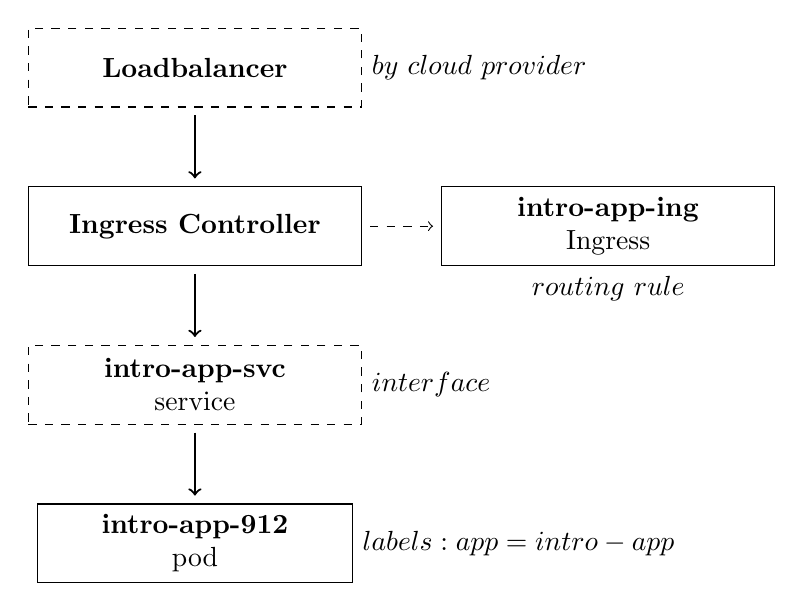
\begin{tikzpicture}
\node[draw, dashed, minimum width=4cm,minimum height=1cm,
      text width=4cm, align=center, label=right:$by\ cloud\ provider$] (LB){\textbf{Loadbalancer}};

\node[draw, minimum width=4cm,minimum height=1cm,
      text width=4cm, align=center] (IC) [below=of LB]  {\textbf{Ingress Controller}};

\node[draw, minimum width=4cm,minimum height=1cm, 
      text width=4cm, align=center,
      label=below:$routing\ rule$] (IR) [right=of IC] {\textbf{intro-app-ing} \\ Ingress};

\node[draw, dashed, minimum width=4cm,minimum height=1cm,
      text width=4cm, align=center,
      label=right:$interface$] (S) [below=of IC] {\textbf{intro-app-svc} \\ service};

\node[draw,minimum width=4cm,minimum height=1cm,
     text width=3cm, align=center,
     label=right:{$labels: app=intro-app$}] (P1) [below=of S] {\textbf{intro-app-912} \\ pod};


\draw [->,thick,shorten >=1mm,shorten <=1mm] (LB.south) -- (IC.north);
\draw [->,dashed,shorten >=1mm,shorten <=1mm] (IC.east) -- (IR.west);
\draw [->,thick,shorten >=1mm,shorten <=1mm] (IC.south) -- (S.north);
\draw [->,thick,shorten >=1mm,shorten <=1mm] (S.south) -- (P1.north);
\end{tikzpicture}
\end{figure}

\smallskip
1. Let's set up the neccessary configuration for already installed \verb|traefik| in the cluster:

\begin{verbatim}
# let's remote the previous service definition
$ kubectl delete -f manifests/kube-service.yaml

# check the files before applying
$ kubectl apply -f  manifests/ingress
\end{verbatim}

\smallskip
2. Let go over the \verb|manifest/ingress/kube-ingress.yaml|:
\inputminted[breaklines]{yaml}{manifests/ingress/kube-ingress.yaml}


\smallskip
3. Now, it is time to call our service. You can print the logs from your pod to verify that the requests are reaching your pod. Let's access our service as our customers would do:

\begin{verbatim}
$ curl --header 'Host: my.app' http://127.0.0.1:8000/echo
\end{verbatim}

\smallskip
4. Now, after verifing that our ingress is working, let's look closer into the ingress:

\begin{verbatim}
# "ing" or "ingress"
$ kubectl get ing
$ kubectl describe ing <ingress name>
\end{verbatim}

\smallskip
5. Let's open a dashboard of our ingress controller - \verb|traefik|:

\begin{verbatim}
$ kubectl get po -n kube-system
$ kubeclt get po -l 'app.kubernetes.io/instance=traefik'
$ kubectl describe po traefik-97b44b794-tf5kf -n kube-system
k port-forward -n kube-system traefik-97b44b794-tf5kf 9000:9000
\end{verbatim}

Open in your browser: \href{http://127.0.0.1:9000/dashboard/}{http://127.0.0.1:9000/dashboard/}, choose \verb|HTTP|, and select our rule from the list.

%%%%%%%%%%%%%%%%
\section{Containers vs Pods}

Please answer the following questions:
\begin{itemize}
\item How many containers can a Pod has?
\item Do containers share disk?
\item Do container share port space?
\item What does \verb|1/1| mean in the output of \verb|kubectl get po|?
\end{itemize}

\bigskip
\bigskip

\section{Fail-over}
Let's see what happens when our application crashes.

\bigskip
1. Open console.

\bigskip
2. Force restart:

\begin{verbatim}
# should work
kill 1

# always works
kill -9 1
\end{verbatim}

Repeat 5 times. Observer the output from: \verb|kubectl get po|.

%
\section{How to debug in nutshell}

Good to ship a minimum of debugging tools in your container, such as, curl or telnet.

Happy debugging path:

\begin{verbatim}
$ kubectl describe ing
$ kubectl describe svc
$ kubectl exec -it <pod name> /bin/bash

# curl, telnet, ...
$ kubectl describe po <pod name>
\end{verbatim}

\begin{verbatim}
$ kubectl logs <pod name>
$ kubectl logs <pod name> -f
$ kubectl logs <pod name> --tail=100
\end{verbatim}

\begin{verbatim}
$ kubectl logs -n kube-system <pod for your ingress controller>
\end{verbatim}

\begin{verbatim}
$ kubectl get events
\end{verbatim}

\bigskip
Notice: To improve the observability, start with monitoring (e.g., Prometheus) and Kubernetes probes (we will cover them later).
%
%
\pagebreak
\section{Kubernetes configmap}

With configmaps, we can deliver values for environment variables or files. Let's change the page in our application:

\bigskip
1. Copy \verb|index.html|:

\begin{verbatim}
$ cp manifests/dockers/site-1.0.0/index.html index.html
\end{verbatim}

\bigskip
2. Edit \verb|index.html| Add your name after the version number:

\begin{verbatim}
<html>
<h1>1.0.0-Natalia</h1>
</html>
\end{verbatim}

\bigskip
3. Let's create a configmap:

\begin{verbatim}
$ kubectl create cm intro-app-index-html --from-file index.html
\end{verbatim}

\bigskip
4. Check the commands:

\begin{verbatim}
# "cm" "configmap"
$ kubectl describe cm intro-app-index-html
$ kubectl get cm intro-app-index-html -o yaml
$ kubectl get cm intro-app-index-html -o json
\end{verbatim}

\pagebreak
5. To make our new index file available, we need to mount it:

\begin{minted}{yaml}
apiVersion: apps/v1
kind: Deployment
metadata:
  name: intro-app-deploy
  labels:
    app_deploy: intro-app
spec:
  replicas: 1
  selector:
    matchLabels:
      app: intro-app
  template:
    metadata:
      labels:
        app: intro-app
    spec:
      containers:
      - name: app
        image: wojciech11/api-status:1.0.0
        ports:
        - containerPort: 80
        volumeMounts:
        - mountPath: "/usr/share/nginx/html"
          name: "html-content"
      volumes:
      - name: html-content
        configMap:
          name: index-html
\end{minted}

\bigskip
5. Let's do a smoke test:

\begin{verbatim}
$ curl --header 'Host: my.app'  "http://127.0.0.1:8000/echo"
\end{verbatim}

\bigskip
6. We can also set environment values, let's create new configmap:

\begin{verbatim}
$ kubectl create configmap intro-app \
  --from-literal=db.name=mydb
\end{verbatim}

\bigskip
7. .. and use it:

\begin{minted}{yaml}
        env:
        - name: DB_NAME
          valueFrom:
            configMapKeyRef:
              name: intro-app
              key: db.name
\end{minted}

\bigskip
8. Open a console in your pods and check whether the ENV variable is set:

\begin{verbatim}
\# printenv | grep DB_NAME
\end{verbatim}

\bigskip
9. More examples you will find in the documentation.

\begin{minted}{yaml}
      envFrom:
      - configMapRef:
          name: db-config
\end{minted}

and the corresponding configmap:

\begin{minted}{yaml}
apiVersion: v1
kind: ConfigMap
metadata:
  name: db-config
  namespace: default
data:
  DB_NAME: mydb
  DB_USERNAME: myuser
\end{minted}

also:

\begin{verbatim}
$ kubectl create configmap intro-app \
    --from-literal=DB_NAME=mydb \
    --from-literal=DB_USERNAME=myuser
\end{verbatim}

\bigskip
Recomendation: Keep everything minimal. 

%%%%%%%%%%%%%%%%%%%%%%%%%%
\section{Kubernetes secret}

Secrets are very similar to configmaps. They provide better security (kind-of) than configmaps.

\bigskip
1. Create a secret with database password:

\begin{verbatim}
$ kubectl create secret generic intro-app-secret \
  --from-literal="db.password=nomoresecrets"
\end{verbatim}

\bigskip
2. Bind it to environment variable in the deployment:

\begin{verbatim}
    env:
      - name: DB_PASSWORD
        valueFrom:
          secretKeyRef:
            name: intro-app-secret
            key: db.password
\end{verbatim}


\bigskip
3. Please deliver \verb|cert.crt| to your application and mount it at \verb|/usr/secet|, find how to do it find on\\ \href{https://kubernetes.io/docs/concepts/configuration/secret/}{kubernetes.io/docs/concepts/configuration/secret/} :

\begin{verbatim}
$ echo "CERT" > cert.crt
$ kubectl create secret generic intro-app-cert --from-file cert.crt
\end{verbatim}

%
\section{Opinionated Configuration}
The configuration and the generation of the kubernetes files is a hot topic.

\begin{markdown}
1. envsubst or similar approaches
2. kustomize
3. Helm
\end{markdown}

\bigskip
1. envsubst or similar approach.

\begin{minted}{yaml}
apiVersion: extensions/v1beta1
kind: Ingress
metadata:
  name: my-extractor
  annotations:
    kubernetes.io/ingress.class: traefik
    traefik.ingress.kubernetes.io/request-modifier: "ReplacePathRegex: /my-app/(.*) /$1"
spec:
  rules:
  - host: ${HOST}
    http:
      paths:
        - path: /extract
          backend:
            serviceName: extractor
            servicePort: 80
\end{minted}

\begin{verbatim}
export HOST=
envsubst < my-k8s.tmpl.yaml > my-k8s.yaml
\end{verbatim}

\bigskip
2. kustomize - overlay
\begin{verbatim}
.
├── base
│   ├── kube-deployment.yaml
│   ├── kube-service.yaml
│   └── kustomization.yaml
├── dev
│   ├── image.yaml
│   ├── kustomization.yaml
│   └── scale.yaml
├── production
│   ├── image.yaml
│   ├── kustomization.yaml
│   └── scale.yaml
└── staging
    ├── image.yaml
    ├── kustomization.yaml
    └── scale.YAML
\end{verbatim}


\bigskip
3. Helm is aiming to become a package manager for Kubernetes.

%
\section{Liveness/Readiness probes}
See \href{https://github.com/wojciech12/talk_zero_downtime_deployment_with_kubernetes}{https://github.com/wojciech12/talk\_zero\_downtime\_deployment\_with\_kubernetes}. Notes:
\bigskip
\bigskip
\bigskip

%
\section{Resource, Limits and QoS}
Notes:

\bigskip
\bigskip
\bigskip

%
\section{RBAC}
See \emph{introduction/ingress-controller/traefik-ingress-controller\_rbac.yaml} and the \emph{Service Account} definition for traefik. Notes:
\bigskip
\bigskip
\bigskip

%
\section{Outlook}
What could be the next steps in learning k8s.

\begin{markdown}

What you could learn next.

Next course *Immediate (Developer)*:

1. Liveness/Readiness probes
2. Monitoring with Prometheus
3. Resource and Limits, QoS for your pods, schedule policies
4. Statefulsets
5. DaemonSets
6. Taints and Tolerations
7. Node affinity 

*Observability plus* with Istio demo as what might the future be:

1. Monitoring
2. Logging
3. Traceability

*Advance (Developer)*:

1. Zero-downtime deployment strategies
2. Horizontal scaling (beta: vertical pod scaling for the pets)
3. Continuous Deployment and Integration
4. TravisCI and Gitlab

*Network and Security*:

1. RBAC deep dive
2. Networking - Internal Loadbalancing - https://kubernetes.io/docs/concepts/services-networking/
3. Restricting Egress/Ingress with [Network Policies](https://kubernetes.io/docs/concepts/services-networking/network-policies/#default-deny-all-egress-traffic)

*Kubernetes customization*

1. Write your first CRD
2. Operators
3. Plugins to kubectl

*CloudNative Ecosystem*

1. Observability: Prometheus stack
2. Observability: EFK
3. Observability: Tracing
4. Ingress Controllers: Traefik, ... , talk about standard and controller-specific annotations
5. Cert-manager
6. Operators for etcd and Vault
7. Kubeless

*More*

1. Istio
2. Operators for ...

*Optionals*

1. Google Kubernetes Engine - GKE
2. Azure Kubernetes Service -  AKS
3. Amazon Elastic Kubernetes - EKS

Trainings and Consultancy: \email{wbarczynski.pro@gmail.com}
\end{markdown}

\end{document}